\documentclass{article}
\usepackage{pdfpages}
\usepackage{float}
\usepackage{enumerate}
\usepackage{amsmath}
\usepackage{amssymb}
\usepackage{graphicx}
\usepackage{url}
\usepackage{subfig}
\usepackage{color}
\usepackage{hyperref}
\usepackage[margin=0.25in]{geometry}
\hypersetup{
    colorlinks=true,
    linktoc=all
}

\title{3GC3 Final Project}
\author{Emily Horsman}
\date{}

\begin{document}

\maketitle

\begin{figure}[H]
    \includegraphics[width=\textwidth]{./examples/Sample100.png}
    \caption{\texttt{examples/Sample.scene} Disks, planes, and spheres demonstrating reflection, refraction, checkered texture mapping, and material configurations. 4x regular sampled anti-aliasing with 100 iterations for soft shadows. 36 hours of CPU time for a 4000x4000px image.}
    \label{fig:title}
\end{figure}

\newpage
\tableofcontents

\section{Feature Overview}

\begin{itemize}
    \item CPU-based ray tracer
    \item Output to PPM bitmaps and a GLUT window
    \item Scene files for configuring rendering and scene parameters, materials, lights, and objects
    \item Support for planes, spheres, and disks
    \item Color and checkered material with proper texture mapping for spheres
    \item Materials specify coefficients for: ambient, diffuse, and specular light; transmission; index of refraction
    \item Multi-threaded rendering with a configurable number of threads
    \item Rudimentary refraction (no Fresnel effect)
    \item Soft shadows achieved by ``jittering'' point lights and averaging multiple renders
    \item Anti-aliasing with both regular (uniform) and random sampling techniques
    \item Adjustable depth-of field and camera field of view
    \item Code documentation from Doxygen in \texttt{html/index.html}
\end{itemize}

\section{Execution}

Running the ray tracer requires a scene file.
The root of this repository includes \texttt{sample.scene} which will be used by default if no scene file is provided.
Running \texttt{make} from the root of the repo will compile and run the ray tracer with the sample scene.
Note that the sample scene file specifies \texttt{threads: 12} by default.
This should be adjusted according to your system.
\\\\
\noindent
The image will be rendered to a PPM bitmap and a GLUT window.
I highly recommend viewing the PPM bitmap, but the GLUT window is convenient for a quick glance.

\subsection{Compile}

\begin{verbatim}
$ make
<…compiling and linking…>
./Ray
=== Render Info ./sample.scene ===
Target              OpenGL, ./sample.ppm
Image Dimension     900 x 700
Threads             12
Max Depth           3
Anti-Aliasing       4
Sampling Method     Regular
Soft Shadows?       No
Iterations          1

Field of View       90
Eye                 0, 0, 0.25
Focal Point         0.5, 0.8, -2
Aperture Radius     Pinhole

Objects             9
Lights              1
\end{verbatim}

\subsection{Unit tests}

There is a small suite of unit tests included.
These primarily cover ray-object intersections.

\begin{verbatim}
$ make test
\end{verbatim}

\subsection{Generating documentation}

This repository uses \texttt{Doxygen} to generate code documentation.
It includes a minimally configured \texttt{Doxyfile}.

\begin{verbatim}
$ make docs
\end{verbatim}

\subsection{Run a scene file}

The \texttt{Ray} executable accepts a single command-line argument for a scene file path.

\begin{verbatim}
$ ./Ray ./examples/DepthOfField.scene
\end{verbatim}

\subsection{Writing a scene file}

Scene files are just plain text files containing sections separated by an extra newline.
The best way to write new ones is to reference \texttt{sample.scene} and \texttt{examples/*.scene}.
\\\\
\noindent
Each section starts with a tag such as \texttt{Renderer} or \texttt{Material}.
A tag is followed by properties in the format of \texttt{key: value}.
Global parameters such as rendering (e.g., number of threads) and camera options (e.g., field of view) are placed under a \texttt{Renderer} and \texttt{Camera} section.
Objects reference materials by an ID you give when writing the material.
You must specify the material section before the objects which use it.
\\\\
\noindent
A minimal sample scene file is produced below.

\begin{verbatim}
Renderer
antiAliasing: 4
samplingMethod: random
useSoftShadows: true
iterations: 30
threads: 12
outputFile: ./minimal.ppm

PointLight
position: 0, 1, -1
radius: 0
intensity: 1

CheckerboardMaterial largeCheckers
color: 1, 1, 1
odd: 0, 0, 0
grain: 0.5
ambient: 0
diffuse: 0.9
specular: 0.1

Plane
material: largeCheckers
point: 0, -1, 0
normal: 0, 1, 0
\end{verbatim}

\noindent
Materials are tagged by their type, followed by their unique ID: \texttt{Material}, \texttt{CheckerboardMaterial}.
Objects are tagged by their type: \texttt{Plane}, \texttt{Sphere}, \texttt{Disk}.
A light is tagged with \texttt{PointLight}.

\subsection{Guidance}

\begin{itemize}
    \item Turning on soft shadows or using a non-zero aperture radius will require setting \texttt{iterations} higher to reduce noise. The precise value depends on the desired quality, effect (sometimes the noise is pleasant, like an artistically chosen film speed in photography), and computational resources.
    \item I've found \texttt{samplingMethod: random} to produce better quality images over \texttt{samplingMethod: regular}.
    \item Objects and lights are placed with $z < 0$. The camera \texttt{eye} is $z > 0$.
    \item Keep soft shadows off and iterations low while testing, and then increase these properties to the desired values.
    \item \texttt{antiAliasing: 4} will improve image quality considerably without much extra render time.
\end{itemize}

\pagebreak

\subsection{Scene file properties}

Enumerations are delimited by pipes \texttt{|}.\\\\

\begin{tabular}{p{0.1\textwidth}llrp{0.4\textwidth}}
    Tag & Property & Type & Example & Description\\
    \hline
    Renderer & width & int & 1200 &\\
    & height & int & 900&\\
    & maxDepth & int & 10 & Maximum recursion depth for specular and transmission rays.\\
    & antiAliasing & int & 16 & Number of anti-aliasing samples per pixel, must be a square number.\\
    & samplingMethod & string & \texttt{regular|random} & The type of anti-aliasing sampling.\\
    & iterations & int & 100 & Render the image for $n$ iterations and average the result.\\
    & threads & int & 4 & Multi-threading.\\
    & useSoftShadows & bool & \texttt{true|false} & Soft shadows will ``jitter'' point lights around their radius.\\
    & outputFile & string & \texttt{./Scene.ppm} & Rendered image path.\\
    \hline
    Camera & fieldOfViewDegrees & int & 45 &\\
    & lookAt & Vec3f & 0.5, 0.5, -2 & Focal point.\\
    & eye & Vec3f & 0, 0, 0.25 & Camera position.\\
    & apertureRadius & float & 0.2 & Use 0 for pinhole/infinite DOF. Higher values have larger DOFs.\\
    \hline
    PointLight & position & Vec3f & 0, 1, -1.5 &\\
    & intensity & float & 0.7 & [0,1]\\
    & radius & float & 0.1 & Must enable soft shadows in \texttt{Renderer}.\\
    \hline
    Material id & color & Vec3f & 1, 0.1, 0.2 &\\
    & ambient & float & 0.1 & [0,1]\\
    & diffuse & float & 0.7 & [0,1]\\
    & specular & float & 0.2 & [0,1]\\
    & transmission & float & 1 & [0,1] From opaque to 100\% transparent.\\
    & refractiveIndex & float & 1.5 & $\eta \geq 1$\\
    \hline
    CheckerboardMaterial id & & & & Shares all \texttt{Material} properties.\\
    & odd & Vec3f & 1, 0, 0 & Color of odd squares. \texttt{color} is for even squares.\\
    & grain & float & 0.5 & Size of checkers.\\
    \hline
    Sphere & origin & Vec3f & 0, 0.5, -1.5 &\\
    & radius & float & 0.5 &\\
    & material & string & blue & Must be a previously tagged material.\\
    \hline
    Plane & point & Vec3f & 0, -1, 0 & Any point in the plane.\\
    & normal & Vec3f & 0, 1, 0 &\\
    & material & string & blue & Must be a previously tagged material.\\
    \hline
    Disk & origin & Vec3f & 0, -1, 0 & Any point in the plane.\\
    & normal & Vec3f & 0, 1, 0 &\\
    & radius & float & 0.05 &\\
    & material & string & blue & Must be a previously tagged material.\\
\end{tabular}

\pagebreak

\section{Depth of Field}

Primary rays normally are generated by casting a ray from a pinhole lens (a single point --- the camera position) through pixels in the image plane.
Call one of these primary rays $\hat{p}$.
This achieves an infinite depth of field.
This ray tracer simulates of depth of field by computing a different primary ray from $\hat{p}$.
\begin{enumerate}
    \item The \texttt{lookAt} property under \texttt{Camera} in your scene file defines the position of the fixed-normal focal plane in the scene. This should be in front of the camera and image plane. \texttt{lookAt} can be conveniently set to the origin of an object you'd like to be in focus.
    \item Find the focal point $f$ by computing the intersection from the eye and direction $\hat{p}$ to the focal plane.
    \item Find the aperture point $a$ by taking the current pixel on the image plane and displacing it by a random amount within the circular aperture (defined with \texttt{apertureRadius} under \texttt{Camera} in your scene file).
    \item Return a new primary ray with origin $a$ and direction $f - a$ (normalized).
\end{enumerate}

\noindent
This process will introduce noise in the image due to the random displacement of the aperture point.
This is solved by rendering multiple iterations and averaging the result to get the final render.

\begin{figure}[H]
    \centering
    \subfloat[\texttt{DepthOfField.scene}]{{ 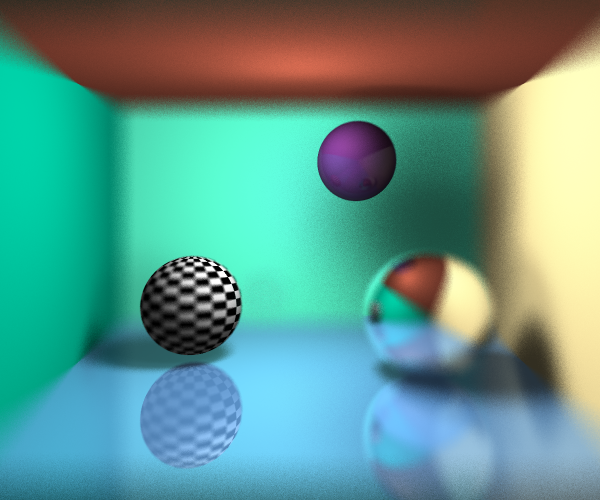
\includegraphics[width=0.45\textwidth]{./examples/DepthOfField.png} }}
    \subfloat[\texttt{DepthOfField2.scene}]{{ 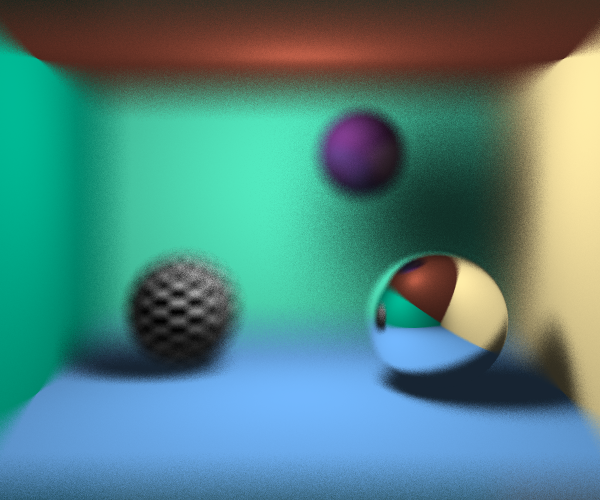
\includegraphics[width=0.45\textwidth]{./examples/DepthOfField2.png} }}
    \caption{A scene displayed with two different focal points and a very shallow depth of field. These renderings have minimal noise reduction applied. It can be increased with the \texttt{iterations} property in the \texttt{Renderer} section of your scene file.}
\end{figure}

\pagebreak

\section{Soft Shadows}

Soft shadows are achieved by randomly displacing each point light within a sphere every time the direction of the light is computed for an intersection point.
The radius of the volume is configured per light.
This technique requires rendering multiple times and averaging the results.
Only non-directional point lights are implemented.
Thus, the direction of a radius $r$ point light at position $\hat{l}$ for an intersection $\hat{p}$ is computed and normalized:
$$
\hat{l} + r * \text{randomVector}(-1, 1) - \hat{p}
$$

\begin{figure}[H]
    \centering
    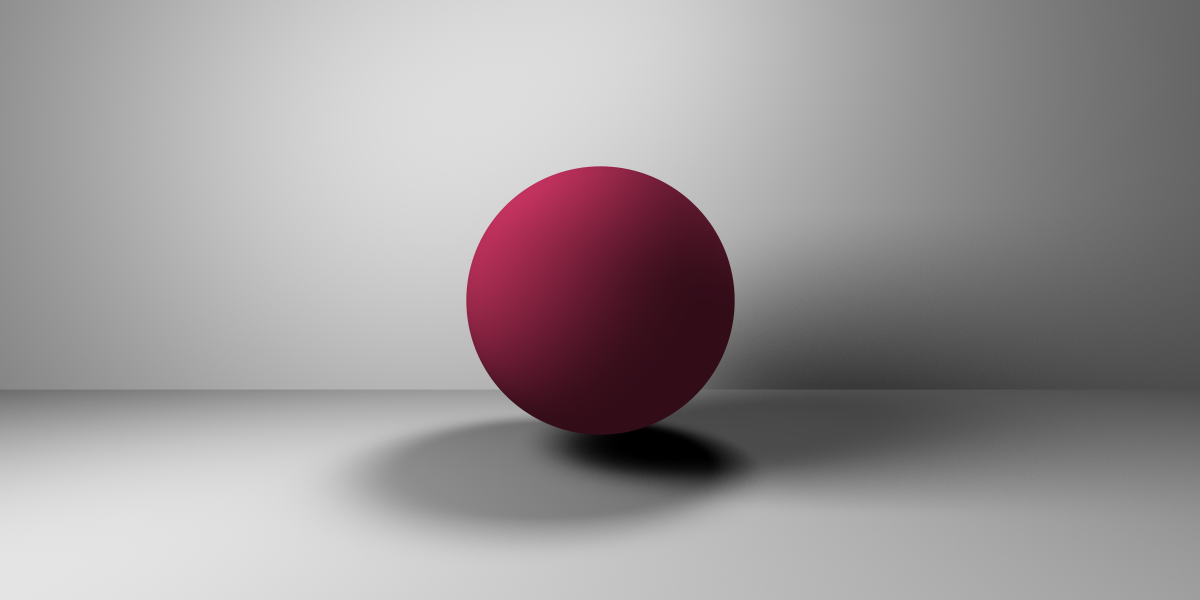
\includegraphics[width=\textwidth]{./examples/SoftShadows.png}
    \caption{\texttt{SoftShadows.scene}. The \texttt{Renderer} section has properties \texttt{useSoftShadows: true} and \texttt{iterations: 500}.}
\end{figure}

\begin{figure}[H]
    \centering
    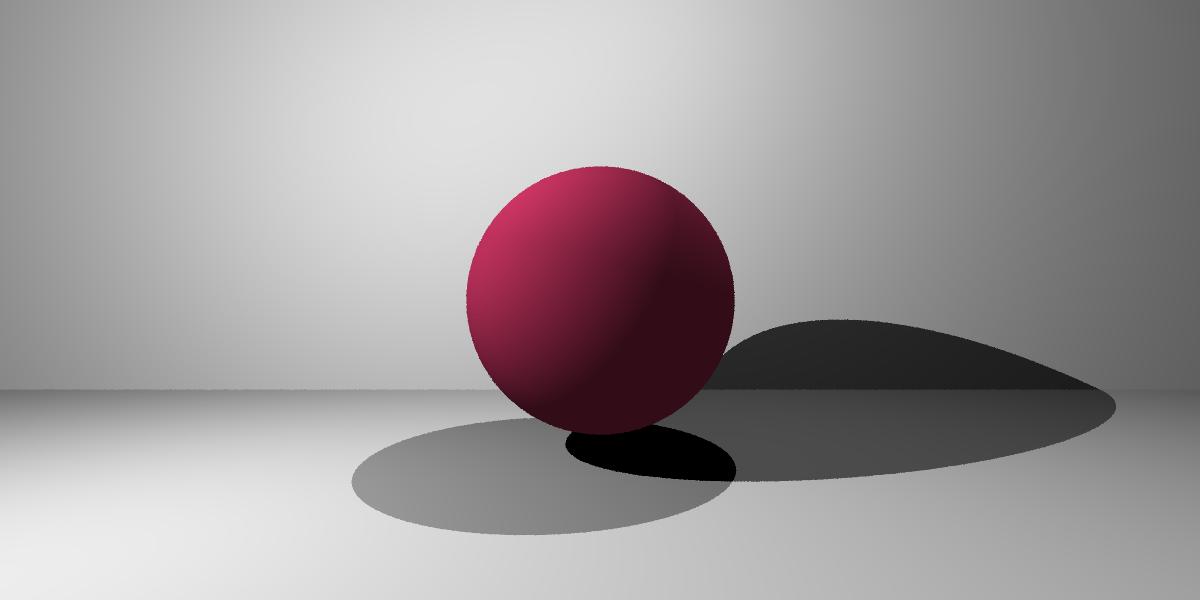
\includegraphics[width=\textwidth]{./examples/SoftShadowsOff.png}
    \caption{\texttt{SoftShadows.scene}. Properties \texttt{useSoftShadows: false} and \texttt{iterations: 1}.}
\end{figure}

\section{Refraction}

\begin{figure}[H]
    \centering
    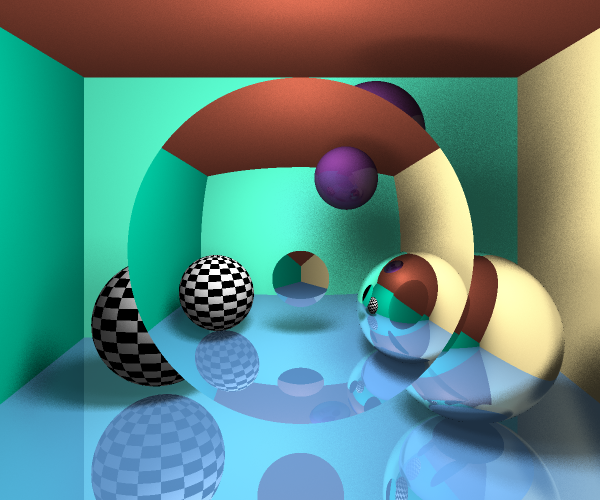
\includegraphics[width=0.6\textwidth]{./examples/DiskLens.png}
    \caption{\texttt{DiskLens.scene}. A 100\% transparent disk with a refractive index of 2.5 placed in front of the scene.}
\end{figure}

\section{Reflection}

\begin{figure}[H]
    \centering
    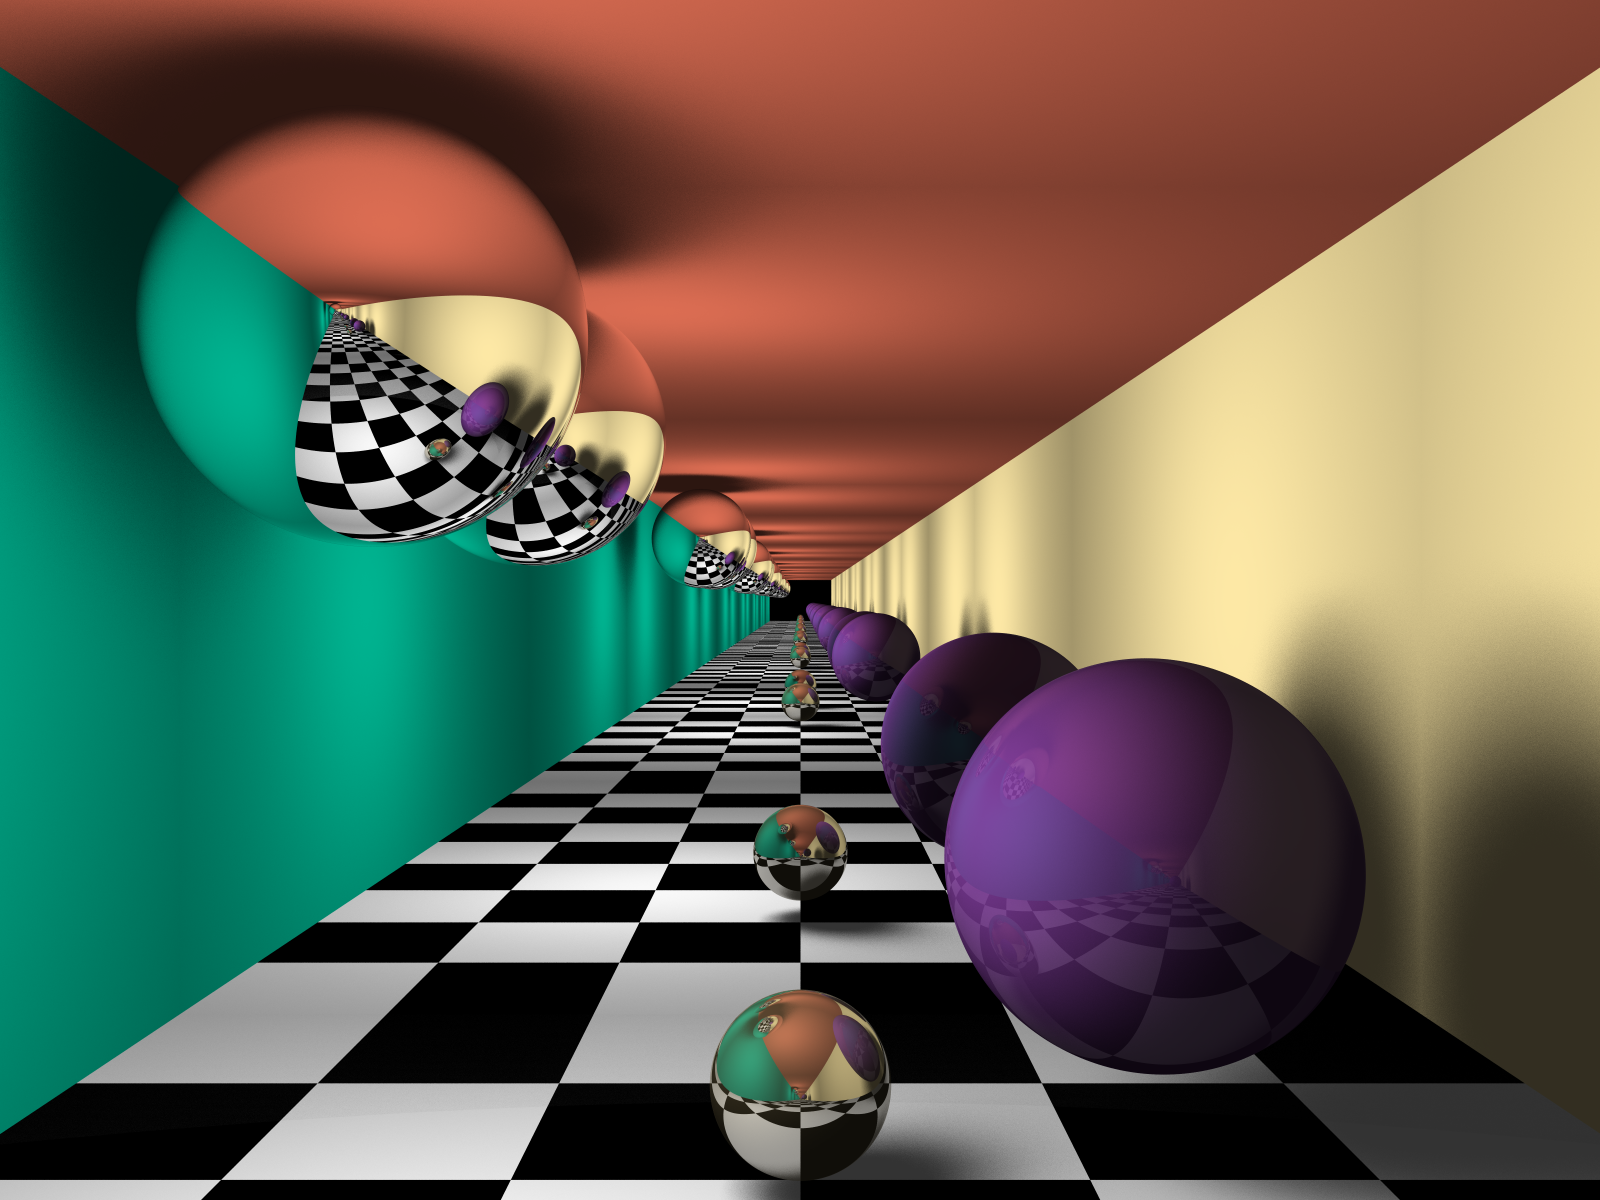
\includegraphics[width=0.6\textwidth]{./examples/HallOfMirrors.png}
    \caption{\texttt{HallOfMirros.scene}. Hall of mirrors with \texttt{maxDepth: 15} under \texttt{Renderer}.}
\end{figure}

\begin{figure}[H]
    \centering
    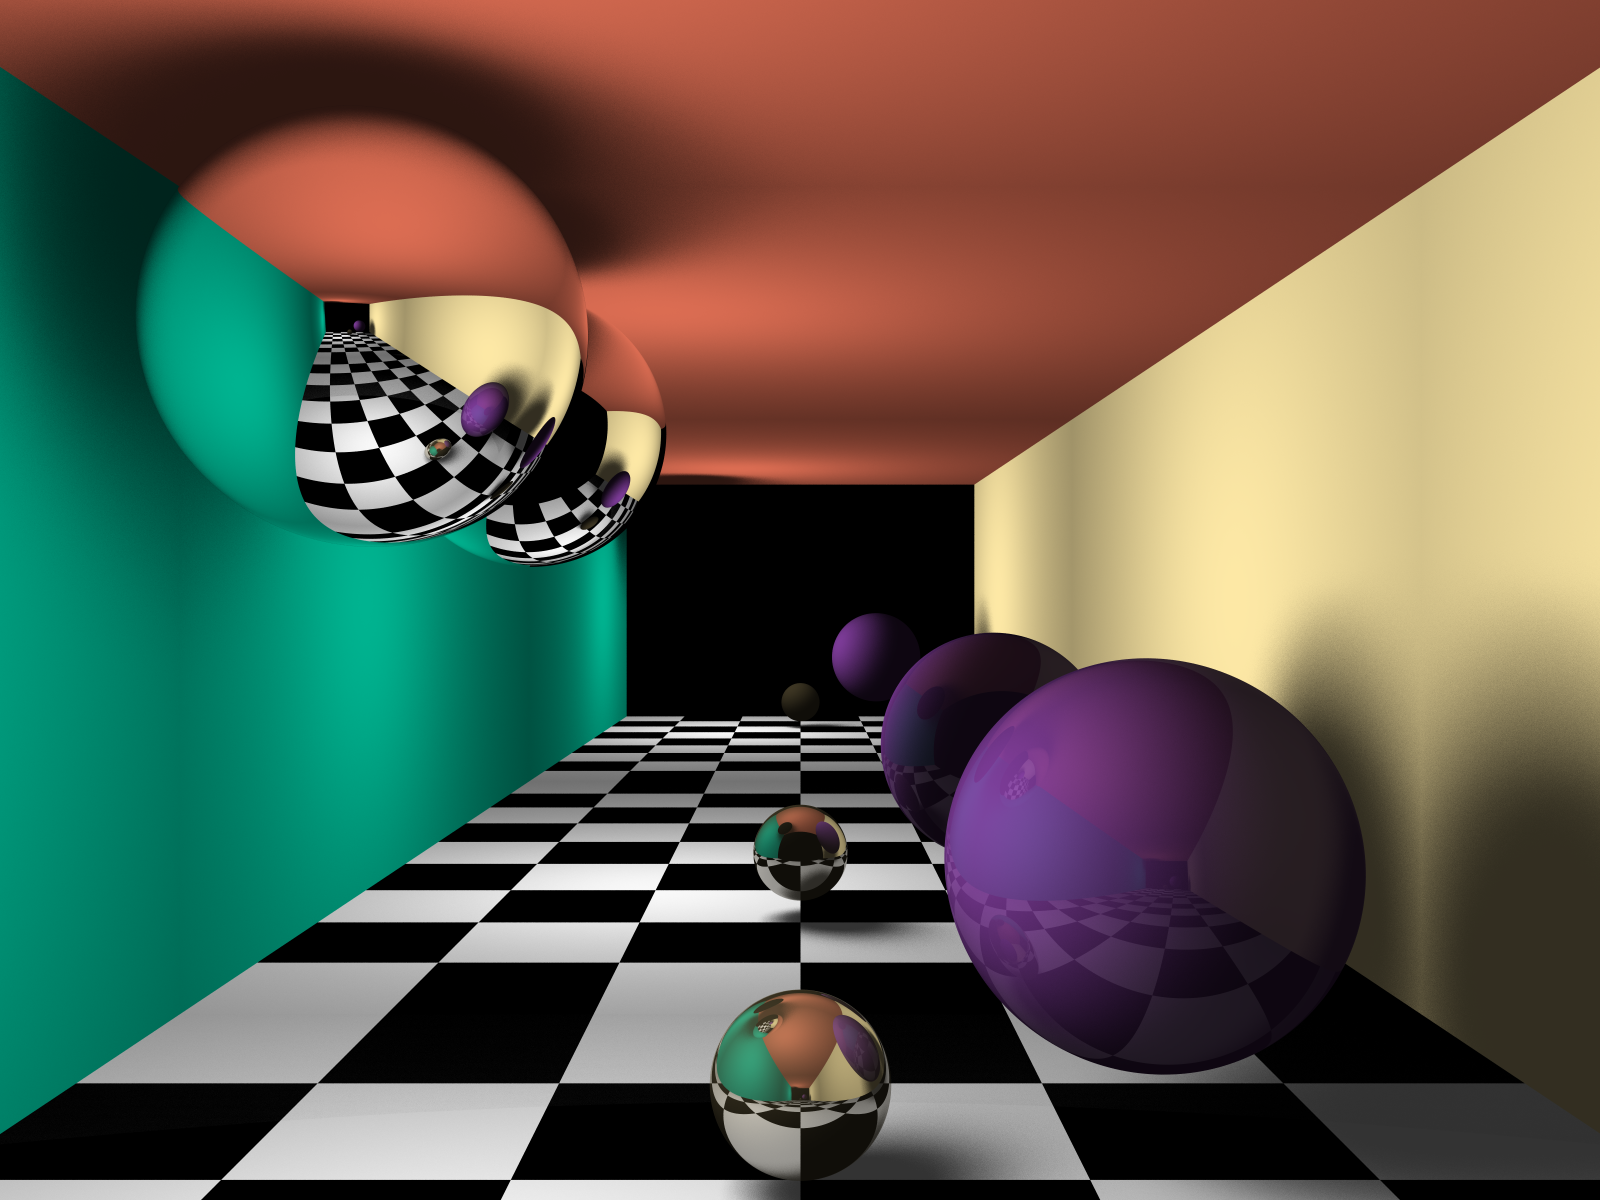
\includegraphics[width=0.6\textwidth]{./examples/HallOfMirrorsDepth2.png}
    \caption{\texttt{HallOfMirros.scene}. Hall of mirrors with \texttt{maxDepth: 2} under \texttt{Renderer}.}
\end{figure}

\begin{figure}[H]
    \centering
    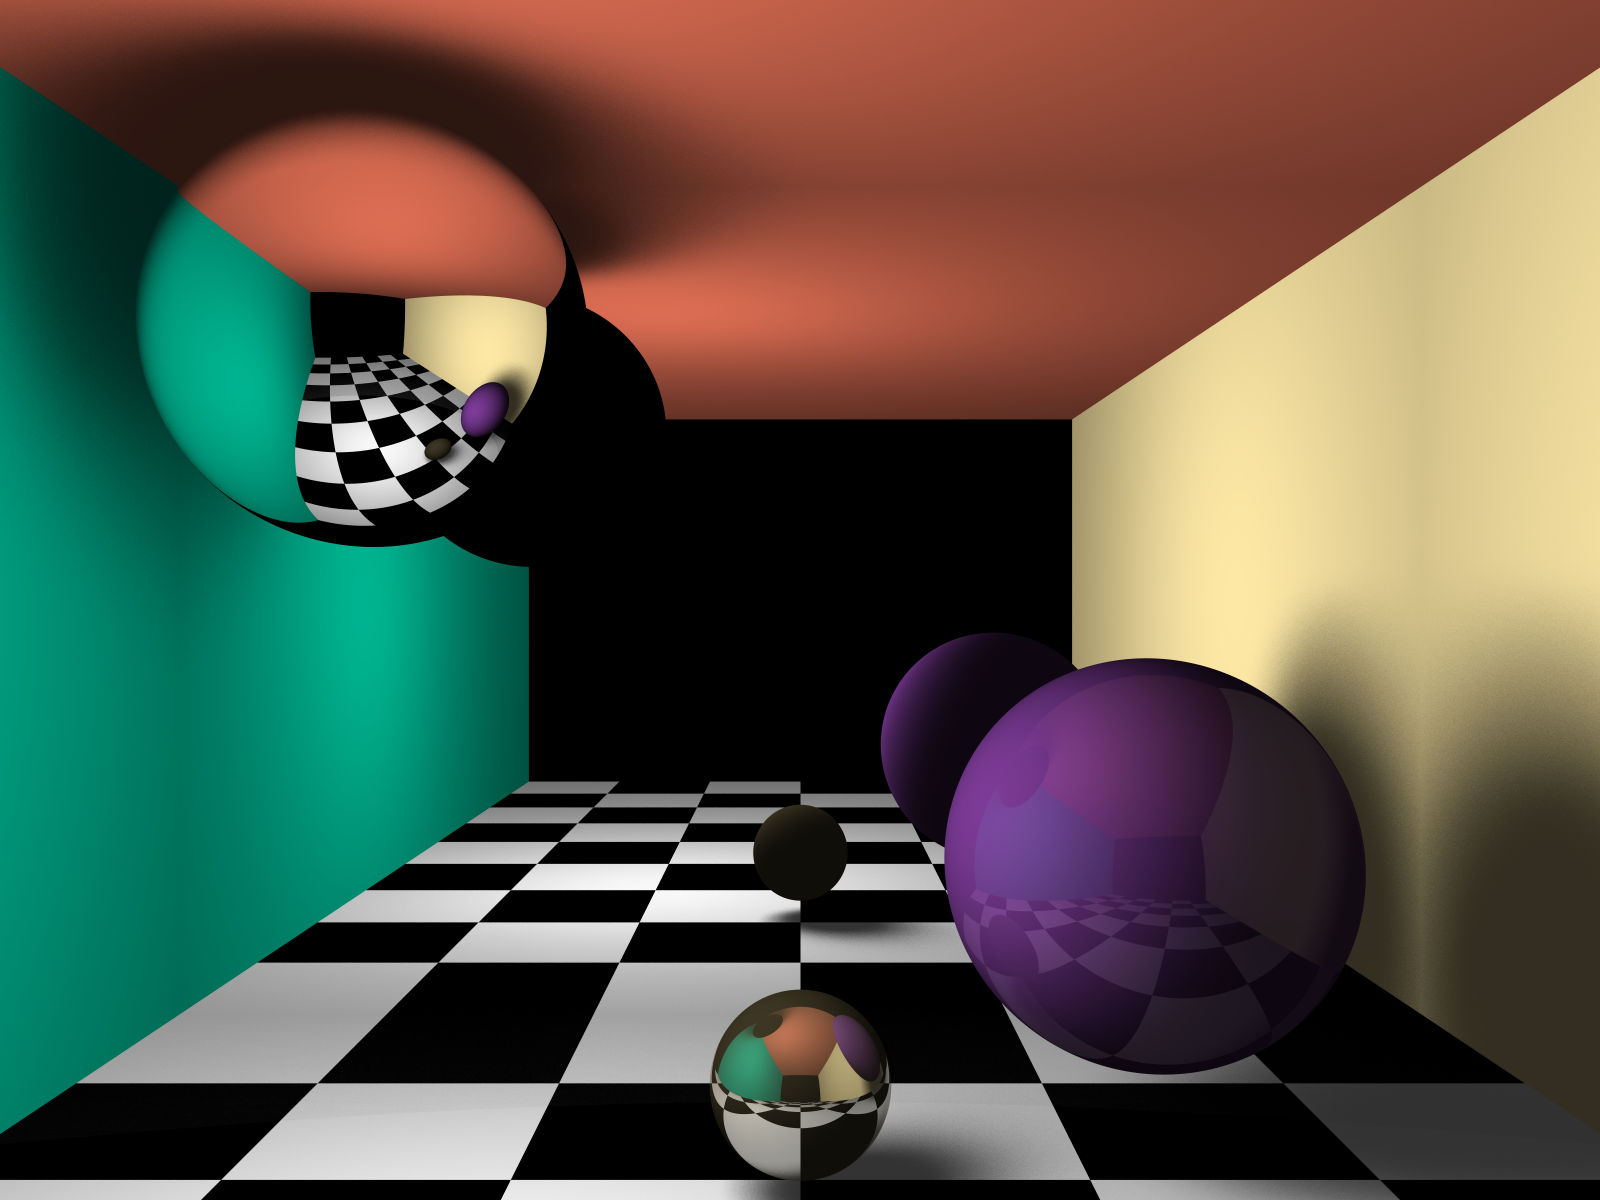
\includegraphics[width=0.6\textwidth]{./examples/HallOfMirrorsDepth3.png}
    \caption{\texttt{HallOfMirros.scene}. Hall of mirrors with \texttt{maxDepth: 1} under \texttt{Renderer}.}
\end{figure}

\section{Anti-Aliasing}

Each pixel of the image is computed with a primary ray cast through the center of the pixel, when \texttt{antiAliasing} is 0 under \texttt{Renderer} in your scene file.
Turning on anti-aliasing makes the renderer trace multiple rays per pixel and then averages the result.
Regular anti-aliasing (\texttt{samplingMethod: regular}) uses a uniform grid with the unit square pixel for its sampling points.
Random anti-aliasing (\texttt{samplingMethod: random}) selects random points within the unit square pixel as its sampling points.
Figure ~\ref{fig:64regular} and ~\ref{fig:64random} show how these two sampling methods look different, particularly in areas of the scene that are very far from the camera.
Without anti-aliasing and with small amounts of regular anti-aliasing, these areas typically look distorted.

\begin{figure}[H]
    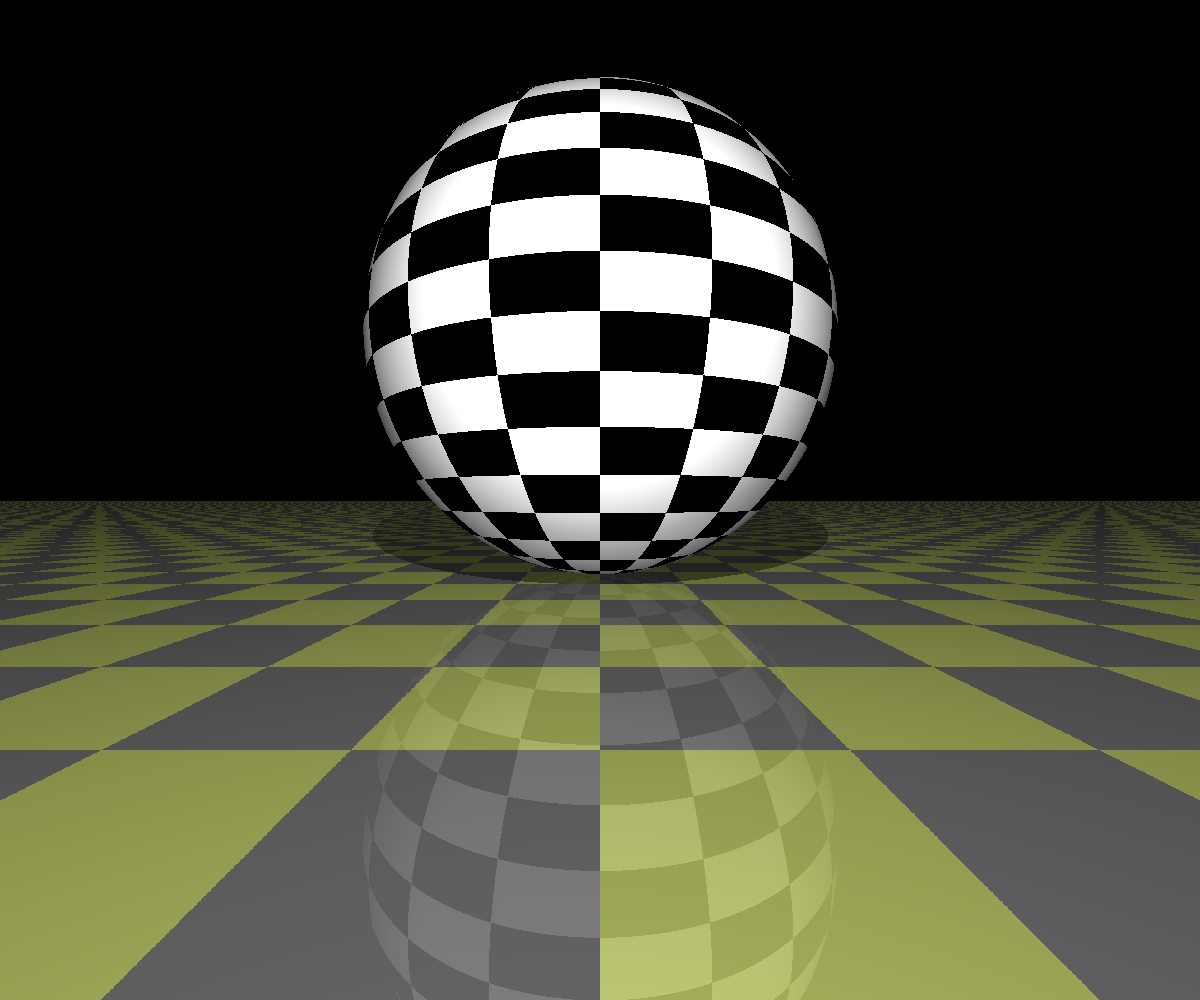
\includegraphics[width=\textwidth]{./examples/AntiAliasingComparison/Scene_noAntiAliasing.png}
    \caption{No anti-aliasing.}
\end{figure}

\begin{figure}[H]
    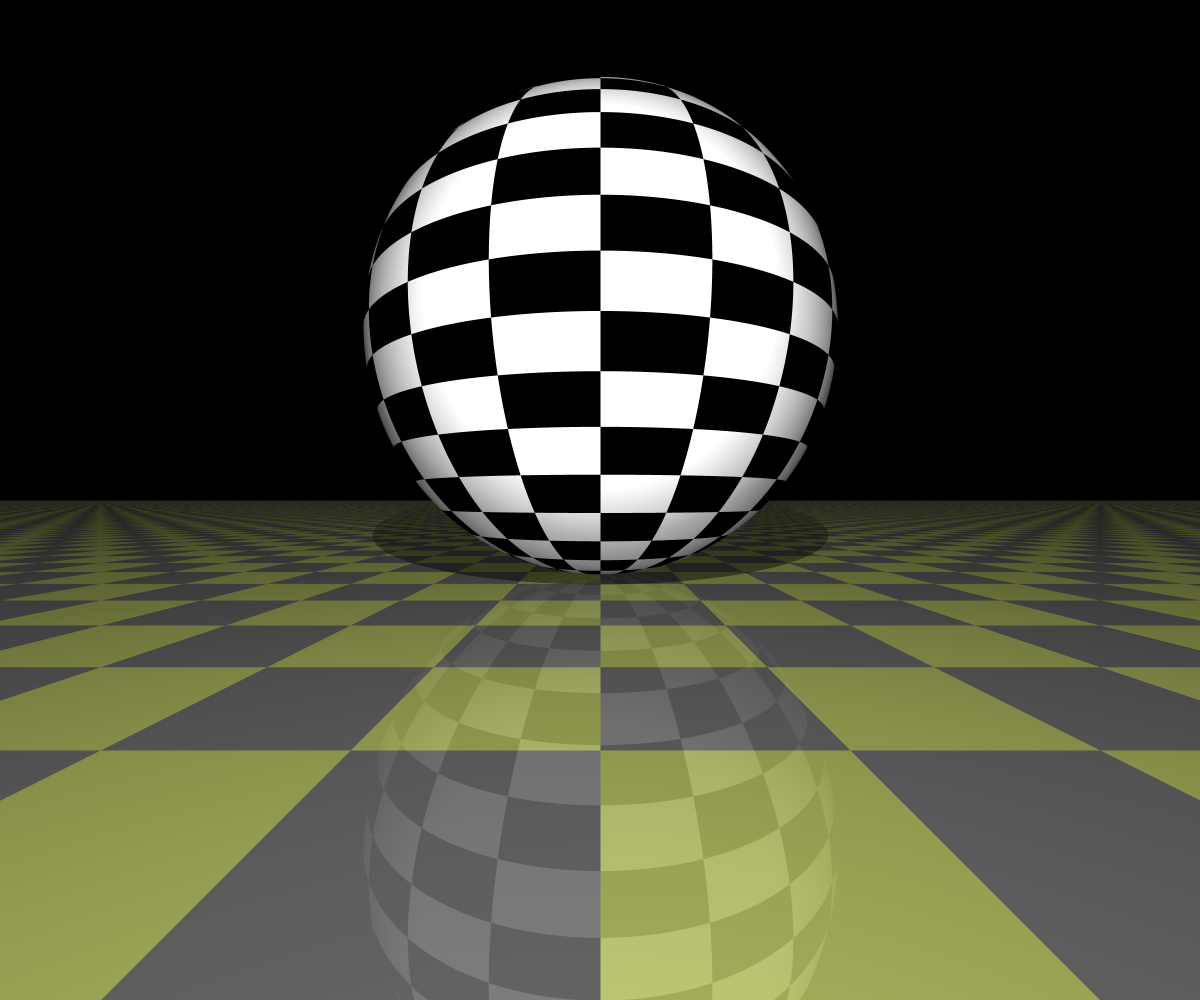
\includegraphics[width=\textwidth]{./examples/AntiAliasingComparison/Scene_regular64.png}
    \caption{64x AA using regular sampling.}
\end{figure}

\begin{figure}[H]
    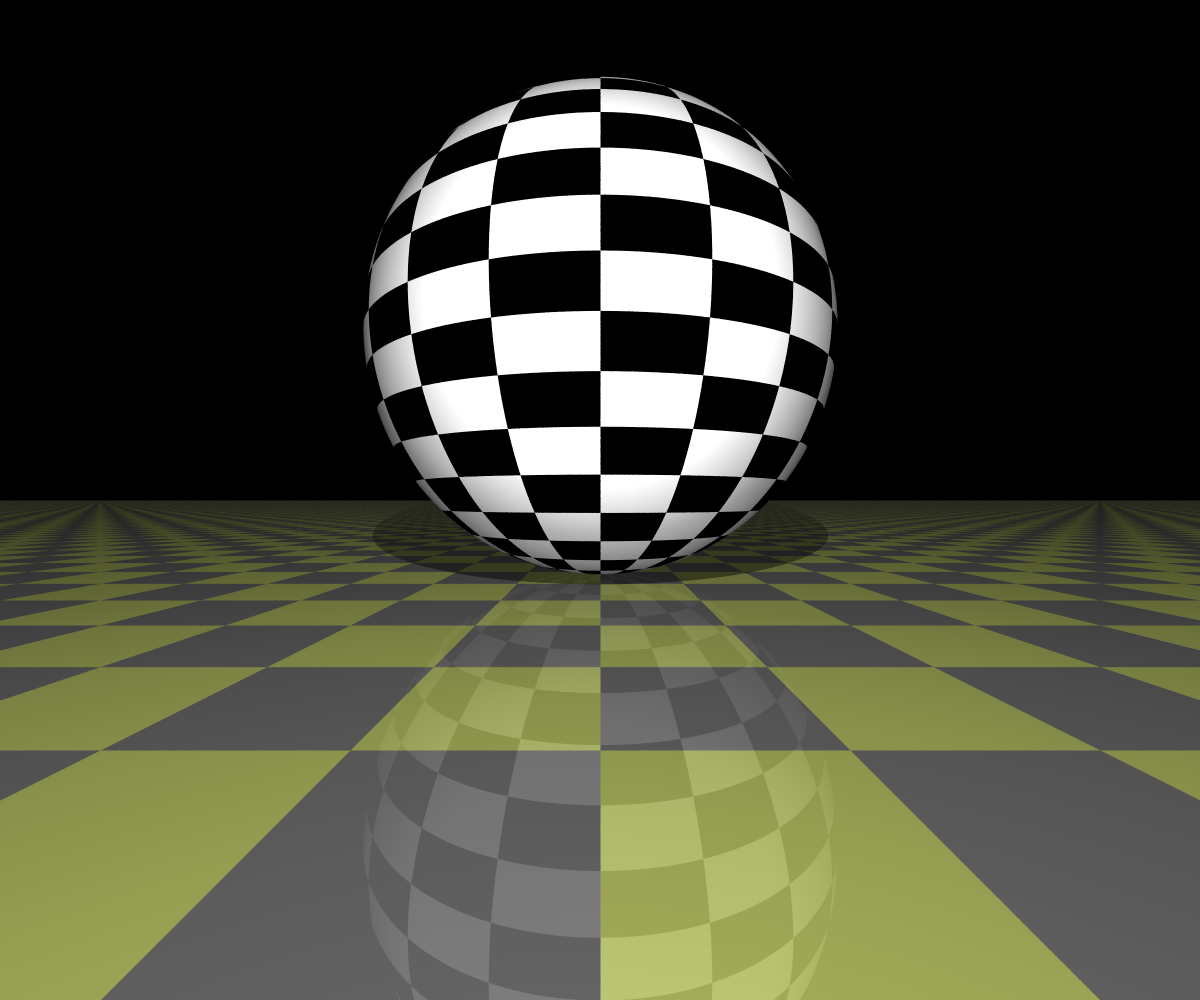
\includegraphics[width=\textwidth]{./examples/AntiAliasingComparison/Scene_random64.png}
    \caption{64x AA using random sampling.}
\end{figure}

\pagebreak

\begin{figure}[H]
    \centering
    \subfloat[Plane]{{ 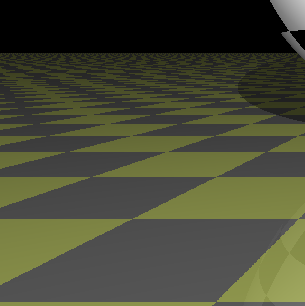
\includegraphics[width=0.3\textwidth]{./examples/AntiAliasingComparison/CheckeredPlane_noAntiAliasing.png} }}
    \subfloat[Sphere]{{ 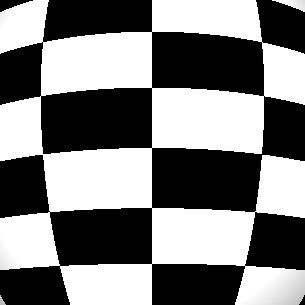
\includegraphics[width=0.3\textwidth]{./examples/AntiAliasingComparison/CheckeredSphereCrop_noAntiAliasing.png} }}
    \caption{Vanishing plane and checkered sphere without anti-aliasing.}
\end{figure}

\begin{figure}[H]
    \centering
    \subfloat[Plane]{{ 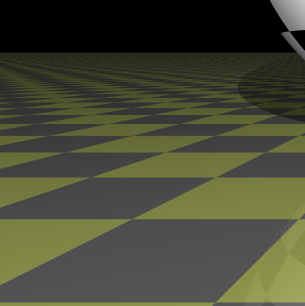
\includegraphics[width=0.3\textwidth]{./examples/AntiAliasingComparison/CheckeredPlane_regular64.png} }}
    \subfloat[Sphere]{{ 
\includegraphics[width=0.3\textwidth]{./examples/AntiAliasingComparison/CheckeredSphereCrop_regular64.png} }}
    \caption{Vanishing plane and checkered sphere with 64x AA using regular sampling.}
    \label{fig:64regular}
\end{figure}

\begin{figure}[H]
    \centering
    \subfloat[Plane]{{ 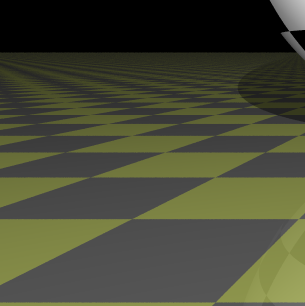
\includegraphics[width=0.3\textwidth]{./examples/AntiAliasingComparison/CheckeredPlane_random64.png} }}
    \subfloat[Sphere]{{ 
\includegraphics[width=0.3\textwidth]{./examples/AntiAliasingComparison/CheckeredSphereCrop_random64.png} }}
    \caption{Vanishing plane and checkered sphere with 64x AA using random sampling.}
    \label{fig:64random}
\end{figure}

\section{Further Scenes}

\begin{figure}[H]
    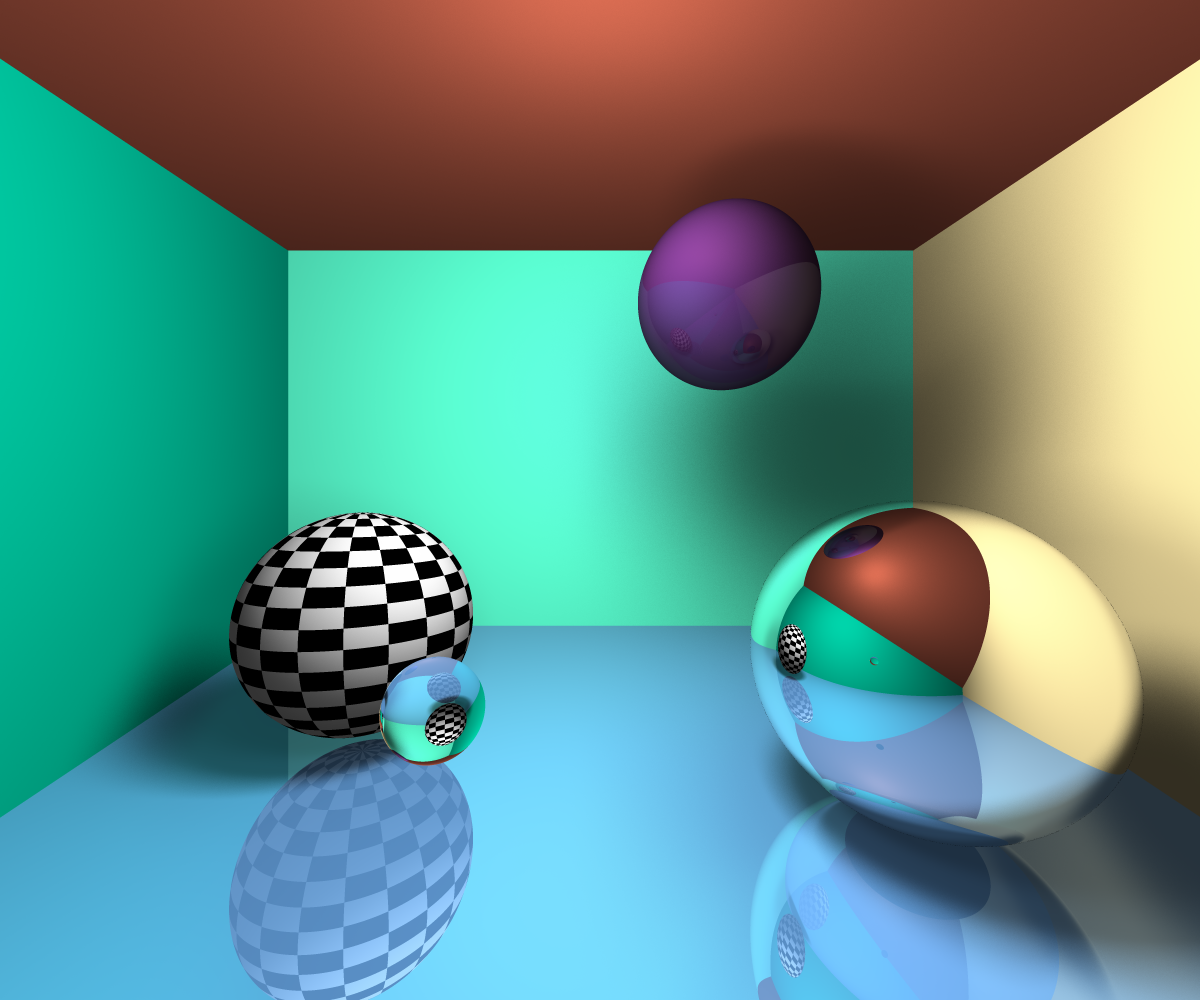
\includegraphics[width=\textwidth]{./examples/SphereRoom.png}
    \caption{Reflective floor, 100\% transparent sphere showing refraction, checkered sphere with texture mapping, mirror sphere. 64x random sampled anti-aliasing with 300 iterations for soft shadows. 13h50m of CPU time.}
\end{figure}

\begin{figure}[H]
    \includegraphics[width=\textwidth]{./examples/Sample1.png}
    \caption{\texttt{examples/Sample.scene} Figure ~\ref{fig:title} run with only a single iteration, \texttt{iterations: 1}}
\end{figure}

\begin{figure}[H]
    \includegraphics[width=\textwidth]{./examples/Sample10.png}
    \caption{\texttt{examples/Sample.scene} Figure ~\ref{fig:title} run with \texttt{iterations: 10}}
\end{figure}


\section{What's Missing?}

These are some things I'd love to do in the future but didn't have time for this semester!

\begin{itemize}
    \item Quadric objects
    \item Fresnel effect
    \item Rendering lights in the scene
    \item 6-DOF camera
    \item Triangles with affine transformations
    \item Mesh files
    \item A regular grid or k-d tree for performance gains
    \item Specular highlights
\end{itemize}

\section{References}

These items are referred to throughout the codebase with \texttt{[n]}.

\begin{enumerate}
    \item https://www.scratchapixel.com/lessons/3d-basic-rendering/ray-tracing-generating-camera-rays/generating-camera-rays
    \item http://www.3dkingdoms.com/weekly/weekly.php?a=2
    \item https://www.scratchapixel.com/lessons/3d-basic-rendering/introduction-to-shading/reflection-refraction-fresnel
    \item https://graphics.stanford.edu/courses/cs148-10-summer/docs/2006--degreve--reflection\_refraction.pdf
    \item Chapter 10 of ``Ray Tracing from the Ground Up'' (Kevin Suffern)
    \item http://cg.skeelogy.com/depth-of-field-using-raytracing/
    \item https://stackoverflow.com/a/13686064/4909532
    \item https://www.scratchapixel.com/lessons/3d-basic-rendering/minimal-ray-tracer-rendering-simple-shapes/ray-sphere-intersection
    \item https://people.cs.clemson.edu/~dhouse/courses/405/notes/texture-maps.pdf
    \item Exercise 18.1 from ``Ray Tracing from the Ground Up'' (Kevin Suffern) p.350
\end{enumerate}

\end{document}
